% --------------------------------------------------------------
% This is all preamble stuff that you don't have to worry about.
% Head down to where it says "Start here"
% --------------------------------------------------------------
 
\documentclass[12pt]{article}
 
\usepackage[margin=0.8in]{geometry} 
\usepackage{hyperref}
\usepackage{url}
\usepackage{xcolor}
\usepackage{array}
\usepackage{biblatex}
\bibliography{bayesian.bib}

\usepackage{dashrule}
\usepackage{multirow}

\usepackage{amsmath,amsthm,amssymb}
\usepackage{turnstile}
\usepackage{mathtools}
\usepackage{bm}
\DeclarePairedDelimiter\ceil{\lceil}{\rceil}

\usepackage{algorithm}
\usepackage[noend]{algpseudocode}
\usepackage{pifont}

\usepackage{graphicx}
\usepackage{subfigure}
\graphicspath{{figs/}}    %change appropriately if required

\newcommand{\x}{\bm{x}}
\newcommand{\bvec}{\bm{b}}
\newcommand{\norm}[1]{\left\lVert#1\right\rVert}
\renewcommand{\algorithmicforall}{\textbf{for each}}
\newlength\myindent % define a new length \myindent
\setlength\myindent{6em} % assign the length 2em to \myindet
\newcommand\bindent{%
  \begingroup % starts a group (to keep changes local)
  \setlength{\itemindent}{\myindent} % set itemindent (algorithmic internally uses a list) to the value of \mylength
  \addtolength{\algorithmicindent}{\myindent} % adds \mylength to the default indentation used by algorithmic
}
\newcommand\eindent{\endgroup} % closes a group

\newenvironment{theorem}[2][Theorem]{\begin{trivlist}
\item[\hskip \labelsep {\bfseries #1}\hskip \labelsep {\bfseries #2.}]}{\end{trivlist}}
\newenvironment{lemma}[2][Lemma]{\begin{trivlist}
\item[\hskip \labelsep {\bfseries #1}\hskip \labelsep {\bfseries #2.}]}{\end{trivlist}}
\newenvironment{exercise}[2][Exercise]{\begin{trivlist}
\item[\hskip \labelsep {\bfseries #1}\hskip \labelsep {\bfseries #2.}]}{\end{trivlist}}
\newenvironment{problem}[2][Problem]{\begin{trivlist}
\item[\hskip \labelsep {\bfseries #1}\hskip \labelsep {\bfseries #2.}]}{\end{trivlist}}
\newenvironment{question}[2][Question]{\begin{trivlist}
\item[\hskip \labelsep {\bfseries #1}\hskip \labelsep {\bfseries #2.}]}{\end{trivlist}}
\newenvironment{prt}[2][Part]{\begin{trivlist}
\item[\hskip \labelsep {\bfseries #1}\hskip \labelsep {\bfseries #2.}]}{\end{trivlist}}
\newenvironment{corollary}[2][Corollary]{\begin{trivlist}
\item[\hskip \labelsep {\bfseries #1}\hskip \labelsep {\bfseries #2.}]}{\end{trivlist}}
\newenvironment{solution}[1][Solution]{\begin{trivlist}
\item[\hskip \labelsep {\bfseries \underline{#1}.} ]}{\end{trivlist}}
\newenvironment{definition}[1][Definition]{\begin{trivlist}
\item[\hskip \labelsep {\bfseries #1.}]}{\end{trivlist}}
 \hypersetup{%
  colorlinks=true,% hyperlinks will be coloured
  linkcolor=blue,% hyperlink text will be green
  linkbordercolor=red,% hyperlink border will be red
}

\begin{document}
 
% --------------------------------------------------------------
%                         Start here
% --------------------------------------------------------------
 
\title{Getting Answers on Stack Exchange\\
\Large{(SDS 384: Bayesian Statistical Methods)}
\date{}%Change
} %if necessary, replace with your course title
\author{Dan Nelson, Shobhit Chaurasia\\
Department of Computer Science}

\maketitle
\hrule

\section{Introduction}
\subsection{Background}
The Stack Exchange network is a network of over 150 question and answer websites, each dedicated to answering questions in a specific field \cite{StackExchange}. The most popular stack exchange website by far is StackOverflow, which is used to ask and answer general questions about programming. However, there are many other exchanges which are also frequented, including the SuperUser exchange for general computer questions, AskUbuntu for those who have questions about Linux, and more. 
 
\subsection{Problem Statement}

The Stack Exchange network posts a data dump from all of its websites quarterly, including detailed information about each post and user. This is a large dataset, ripe for drawing interesting conclusions. Computer scientists often use StackOverflow to get answers to difficult coding questions; because of this we decided to analyze what factors determine the length of time it takes between posting a question on StackExchange and getting that question answered. Ideally, if we can understand these factors, then it becomes easier to get a question answered.


\section{Dataset}

The stack exchange data dump is split up by each individual stack exchange. For speed of analysis, we selected the Academia and Data Science stack exchanges. The Academia Exchange is a forum for posting general questions about working in Academia. The Data Science stack exchange is used for posting questions about Data Science topics, which can vary across programming, statistics, and other fields. These two exchanges have 6134 and 801 questions, respectively. Each question in a given exchange has a timestamp for when it is posted, and a timestamp for when it is answered. We calculated the difference between these two times in seconds, which is the time to answer a question after it has been posted, then used predicting that value for a given question as the goal for each model constructed.

 \begin{figure}[h]
  \centering
  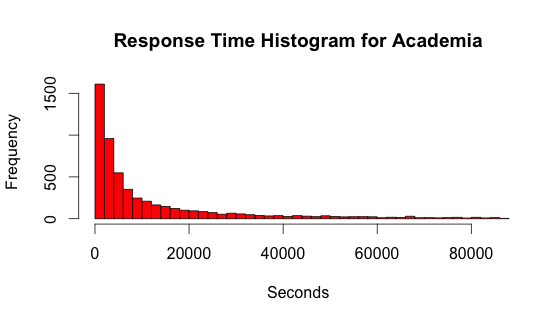
\includegraphics[scale = 0.5]{academia_histogram.png}
  \caption{Time to Answer in Academia Exchange}
  \label{academia_hist}
\end{figure}

Initial visualization of the data allows viewing the distribution of response times for each stack exchange. These two visualizations illustrate a histogram of all response times for each exchange, truncated at 86400 seconds (1 day). It is apparent from Figure $\ref{ds_hist}$ that the data science histogram has a fatter tail of waiting times. Indeed, when comparing the two datasets, only 68\% of the probability mass of the data science stack exchange has a response time of less than 1 day, whereas 89\% of the probability mass of the Academia stack exchange has a response time of less than 1 day. This provides support for later hierarchical approaches that we take to modeling this data. 



\begin{figure}[h]
  \centering
  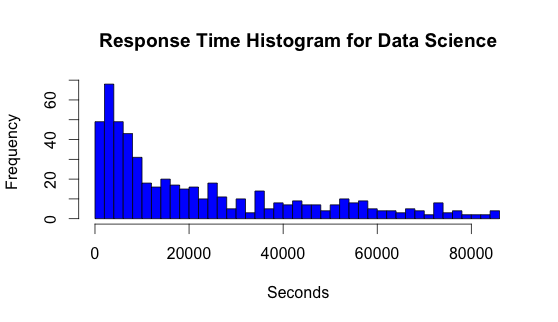
\includegraphics[scale = 0.5]{data_science_histogram.png}
  \caption{Time to Answer in Data Science Exchange}
  \label{ds_hist}
\end{figure}


For each question, the data dump provides up to 64 different features. We selected a subset of these which we believed to be relevant and interesting for analyzing this data. Four of the features we chose to analyze are features specific to a given post, and they are listed in Table $\ref{post_feats}$. Four of the features we chose to analyze are specific to the user who actually made a given post, and they are listed in Table $\ref{user_feats}$. 

\begin{table*}[ht]
  \centering
  \begin{tabular}{|c|c|}\hline
    Question Feature & Description \\ \hline
    Views & Number of views for a question \\
    Score & Question upvotes - downvotes \\
    Comments & Number of comments on the question\\
    Favorites & Number of favorites for question\\ \hline
  \end{tabular}
  \caption{Post-Specific Features}
  \label{post_feats}
\end{table*}

\begin{table*}[ht]
  \centering
  \begin{tabular}{|c|c|}\hline
    User Feature & Description \\ \hline
    Reputation & Reputation of posting user \\
    User views & Views for all of user's posts \\
    Upvotes & Number of upvotes given by user \\
    Downvotes & Number of downvotes given by user \\ \hline
  \end{tabular}
  \caption{User-Specific Features}
  \label{user_feats}
\end{table*}


\section{Methodology}
We implemented our models using Stan \cite{stan}, a toolkit for Bayesian MCMC analysis supported in both R and Python. Data cleaning was done in Python, and Stan models were created in both R and Python. 

\section{Models}
\subsection{Ordinary Least Squares Regression}
The go-to model to kick start any predictive modeling task that involves regression is the Ordinary Least Squares Regression, in part due to its simplicity and speed. The model takes the form of a simple linear equation, given by:
\begin{align*}
y=X\beta
\end{align*}
where $y$ denotes the response variable to be predicted (in our case, the response time), and $X$ represents the feature matrix (often referred to as the \textit{design matrix} in Statistics jargon), containing the values for the explanatory variables (also called co-variates, or features).

Before fitting the linear model to our data, we observed that the scale of values taken by different features varied wildly - response times being of the order of tens of thousands, while number of views being of the order of thousands, and comments count generally taking small values in single or double digits. As a pre-processing step, we standardized the values for all the features and the response variables, by transforming them to have zero mean and unit variance. Not only does this aid the regression model to infer a better fit for the data, it also enables direct comparison of the coefficients across features to asses feature importance.

Two data aggregation schemes were employed for fitting the model. The first involved fitting a common model to the pooled dataset from the two Stack Exchanges. The second involved fitting separate regression models to the data from the two Stack Exchanges, treating the two as independent of each other. Results for both the schemes are reported in Table. \ref{table:ols-rmse}. Note that the RMSE errors are also in the scale of the transformed variables; hence, these values might cannot be directly compared to RMSE values for few other models that are described later in which feature transformation is not used (such as Generalized Linear Model). 

\begin{table*}[ht]
  \centering
  \begin{tabular}{|c|c|c|}\hline
    Model & Data Science RMSE & Academia RMSE   \\ \hline
    OLS (Un-Pooled) & 0.9992 & 1.0008 \\ \hline
    OLS (Pooled) & \multicolumn{2}{c|}{1.0003} \\ \hline
  \end{tabular}
  \caption{RMSE error}
  \label{table:ols-rmse}
\end{table*}

RMSE for Data Science is lower for the un-pooled model, suggesting that pooling together data from both the Stack Exchanges does not go well with the predictions for the Data Science Stack Exchange. The reason for this could be attributed to the imbalance in the number of observations coming from the two Stack Exchanges, and the differences in the underlying patterns in the data. Data Science is a fairly dormant Stack Exchange with fewer active users as compared to Academia. As a result, the response times are larger (as seen in Fig. \ref{ds_hist}). However, the larger size of the Academia dataset sways the model towards learning coefficients that are more compatible with the Academia dataset, overshadowing the contribution from the Data Science dataset.

\begin{table*}[ht]
  \centering
  \begin{tabular}{|c|c|c|}\hline
    Covariate & Coefficient Estimate & Coefficient SE \\ \hline
    Intercept & -0.01 & 0.01\\
    View Count & -0.015 & 0.01 \\
    Score & 0.022 & 0.02 \\
    Comment Count & 0.044 & 0.01 \\
    Favorite Count & -0.005 & 0.01 \\
    Views (User) & 0.002 & 0.004 \\
    Downvotes (User) & 0.005 & 0.003 \\
    Reputation (User) & 0 & 0.003 \\
    Upvotes (User) & 0.001 & 0.003 \\ \hline
  \end{tabular}
  \caption{Coefficients for Pooled OLS Regression model}
  \label{table:ols-coeff}
\end{table*}

The coefficient values for this model are reported in Table. \ref{table:ols-coeff}. We can use the magnitude and sign of the coefficients as a proxy for the impact of features on the response times. Score and Comment Count seem to have the maximum impact, while user related features do not have a significant contribution to the regression output.

\subsection{Bayesian Linear Regression}
A natural extension of the Ordinary Least Squares model is its Bayesian counter-part: the Bayesian Linear Regression model. In this model, instead of working with point estimates of the response times and the coefficient values, we also model the uncertainties in their values. The core prediction function is still linear, but we allow for the predictions to have noise, modeled as a Gaussian centered around the predictions' point-estimates.

\begin{align*}
y &=X\beta + \text{noise} \\
y &\sim \text{Normal}(X\beta, \epsilon) \\
\beta_i &\sim \text{Norma}(0, 100) \\
\epsilon &\sim \text{Uniform}(0,5)
\end{align*}

We chose non-informative ``flat'' prior for the coefficients $\beta_i$, approximated by a zero-mean, high variance Normal. Given the scale of the response variable $y$, the noise captured by the standard deviation, $\epsilon$ of the Normal was also given a flat Uniform prior on $\left[0, 5\right]$. As with the OLS regression, all the features and the response times were standardized before fitting the model to the data.

As with OLS regression, we can imagine two data aggregation schemes - pooled and un-pooled. The first involved pooling together data from both the Stack Exchanges, and fitting a common model on the aggregated dataset. The second scheme involved treating the two forums as completely independent, and fitting separate  models to each of them. Results for Bayesian Linear Regression fit with the pooling scheme are reported in Table. \ref{table:bayesian-regression-rmse}. As expected, the RMSE value is lower for this model as compared to that for OLS Regression model.

\begin{table*}[ht]
  \centering
  \begin{tabular}{|c|c|c|}\hline
    Model & Data Science RMSE & Academia RMSE   \\ \hline
    Bayesian Regression (Pooled) & \multicolumn{2}{c|}{0.9054} \\ \hline
  \end{tabular}
  \caption{RMSE error}
  \label{table:bayesian-regression-rmse}
\end{table*}

Since Bayesian Regression model allows us to model the distribution over the parameters (coefficients and the error term), we can compare the contribution of different features through the distributions of their coefficients, and the resulting credible regions, instead of relying solely on their point estimates. Fig. \ref{fig:bayesian-credible} shows the posterior distributions for the coefficients. The results are consisted with those of the OLS Regression model. The coefficients corresponding to user-related features ($b[5]-b[9]$) are largely irrelevant, because of their low magnitudes. Not only do their point-estimates (mean) have low magnitudes, their $95\%$ credible regions are narrow as well, further strengthening the observation that user-related features do not have significant impact on response times. The Comment Count has the maximum influence, and this influence is positive, indicating that a higher Comment Count increases the response time for that question. As discussed later, this might be attributed to ill-specified questions requiring further clarification through comments before an informed answer can be posted for that question, thereby increasing its response time. The posterior distributions for Favorite Count presents a quintessential illustration of how the richness of the Bayesian Regression setting trumps the simplicity of the frequentist OLS Regression setting. While the OLS Regression model estimates a negative influence of the Favorite Count towards the response time (higher Favorite Count driving the response times higher), we can see that this point-estimate fails to capture the uncertainty associated in the inference. The $95\%$ credible region for Favorite Count ($b[5]$) indeed has a wide credible region that does cross over to the positive side.

The side-effects of the no-pooling scheme can be seen in Fig. \ref{fig:bayesian-unpooled-credible} where the estimates for Data Science are wildly different from that of Academia. While we do expect the two forums to have nuanced differences in their characteristics, we also expect similarity at an abstract level, like general un-relatedness of user-specific parameters to response times. However, as is apparent in Fig. \ref{fig:bayesian-unpooled-credible}, this general agreement is missing. This might be an artifact of the small size of the Data Science dataset, which might result in unreliable posterior estimates. This can be fixed by letting the data-scarce Regression model for Data Science borrow some strength from the data-rich Academia model, without enforcing a common model on both the groups, an idea that is pursued in the next model we used - Hierarchical Linear Regression.

\begin{figure}[p]
  \centering
  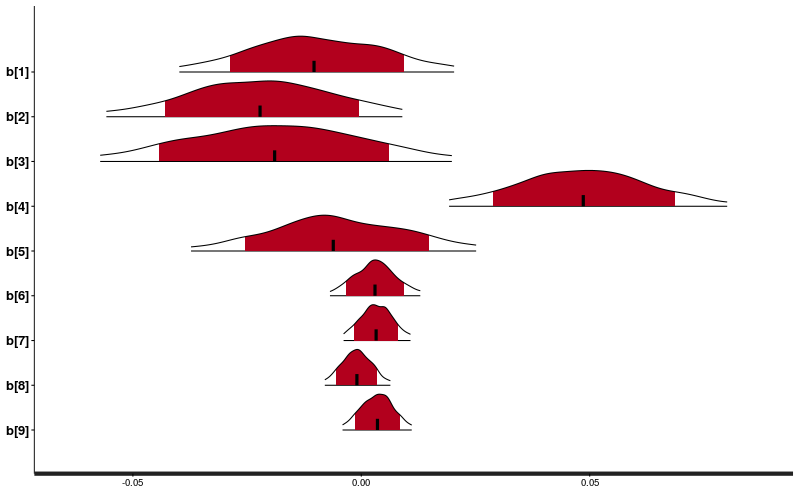
\includegraphics[scale = 0.5]{figs/bayesian-credible-regions.png}
  \caption{Posterior distributions for $\beta$ values for pooled Bayesian Regression model using complete-pooling scheme. The outer interval shows the $95\%$ credible region, while the inner, shaded interval corresponds to $80\%$ credible region.}
  \label{fig:bayesian-credible}
\end{figure}

\begin{figure}[p]
\centering
	\subfigure[Academia] 
    {
		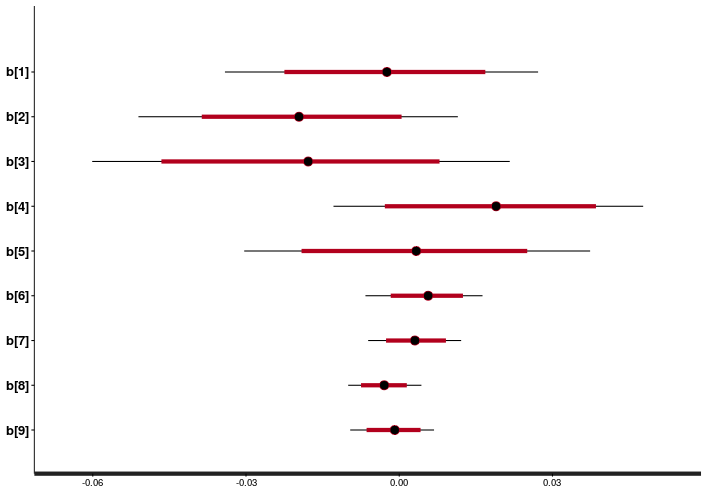
\includegraphics[width=0.43\textwidth]{figs/bayesian-1}
	}
  \subfigure[Data Science] 
  {
      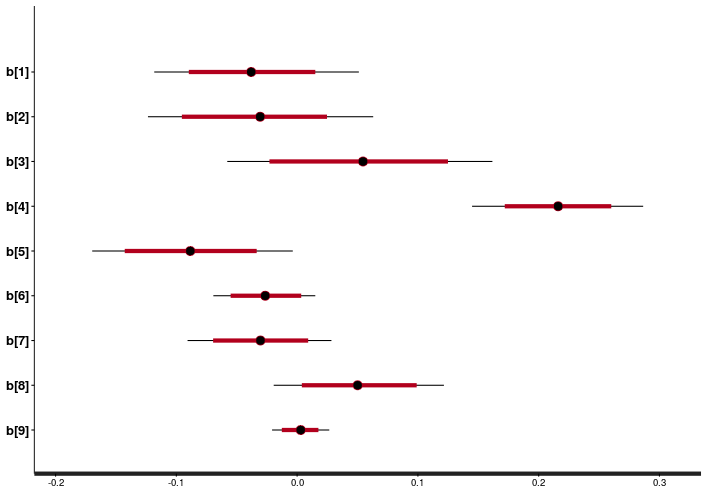
\includegraphics[width=0.43\textwidth]{figs/bayesian-2}
  }
\caption{Posterior credible regions for $\beta$ values for Bayesian Regression model using no-pooling scheme. The outer interval shows the $95\%$ credible region, while the inner, shaded interval corresponds to $80\%$ credible region.}
\label{fig:bayesian-unpooled-credible}
\end{figure}

\subsection{Hierarchical Linear Regression}
The Bayesian reasoning exploited in the Bayesian Regression model with pooling can be extended to the un-pooled scheme, with even more richness. Instead of treating the two Stack Exchanges as completely independent of each other, and fitting separate Bayesian Regression models to each, we can connect the two models through group-level parameters. This provides a balance between the two extremes we have seen so far - complete pooling, where observations from different groups are treated identically, and no-pooling, where observations from different groups are treated independently. Hierarchical Regression takes a middle ground by connecting the two groups at an ``abstract level''. This involves setting up a hierarchy, which is specified in the form described below. The subscript $g$ indicates separate parameters for each group (each Stack Exchange).

\begin{align*}
y &=X\beta_g + \text{noise}_g \\
y &\sim \text{Normal}(X\beta_g, \epsilon_g) \\
\epsilon_g &\sim \text{Uniform}(0,5) \\
\beta_{i,g} &\sim \text{Norma}(\mu_b, \sigma_b) \\
\mu_b &\sim \text{Normal}(0, 100) \\
\sigma_b &\sim \text{Uniform}(0, 100)
\end{align*}

At the lower level of the hierarchy, a separate Bayesian Regression model is fit to each of the Stack Exchange, with each model having separate parameters ($\epsilon_g$ and $\beta_{:, g}$). However, unlike the complete un-pooled setting where these parameters are independent of each other, in the Hierarchical Regression setting, the group level parameters borrow strength across the groups by being connected at the second level in the hierarchy through a common distribution (Normal($\mu_b$, $\sigma_b$). The parameters for this ``unifying'' distribution either be given point estimates, or an informative/vague prior of their own, thereby adding another level to the hierarchy. We can go as high as we want; however, one should note that going higher up the hierarchy the obscures the original problem at hand.

The RMSE value for this model is reported in Table. \ref{table:hierarchical-regression-rmse}. While there is a small improvement in RMSE as compared to the pooled Bayesian Linear Regression setting, the more interesting observation is the shrinkage of coefficient estimates (Fig. \ref{fig:hierarchical-credible}) for the two groups (compared to Fig. \ref{fig:bayesian-unpooled-credible}), indicating that the Hierarchical setting compensates for the extreme nature of no-pooling scheme by letting the parameters borrow some strength from their counter-parts in other groups. This is especially true for the Data Science Stack Exchange where the observations are fewer, and hence the estimates with no-pooling schemes are likely to be unreliable, and no in-sync with the ``general scheme of things''.

\begin{table*}[ht]
  \centering
  \begin{tabular}{|c|c|c|}\hline
    Model & Data Science RMSE & Academia RMSE   \\ \hline
    Hierarchical Regression & \multicolumn{2}{c|}{0.9050} \\ \hline
  \end{tabular}
  \caption{RMSE error}
  \label{table:hierarchical-regression-rmse}
\end{table*}

\begin{figure}[ht]
\centering
	\subfigure[Academia] 
    {
		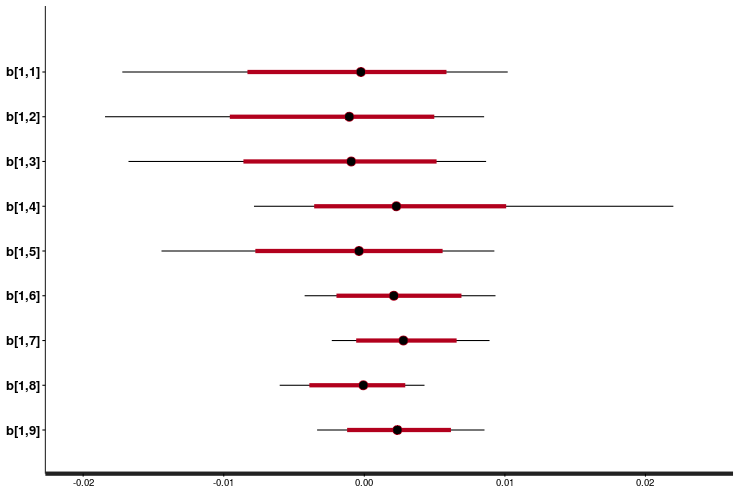
\includegraphics[width=0.43\textwidth]{figs/hierarchical-1}
	}
  \subfigure[Data Science] 
  {
      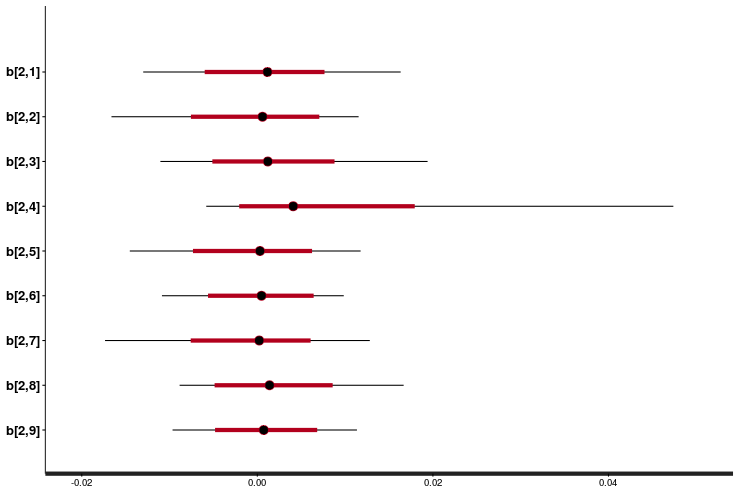
\includegraphics[width=0.43\textwidth]{figs/hierarchical-2}
  }
\caption{Posterior credible regions for $\beta$ values for Hierarchical Linear Regression model. The outer interval shows the $95\%$ credible region, while the inner, shaded interval corresponds to $80\%$ credible region.}
\label{fig:hierarchical-credible}
\end{figure}

\subsection{Generalized Linear Model}
A generalized linear model is similar to a linear regression, except it is assumed that the relationship between the covariates and the dependent variable is not linear. Rather, the model takes the form:
\begin{align*}
E(y|X) &= g^{-1}(X\beta) + \phi
\end{align*}

Thus, the covariates and the dependent variable are linked together through $g(X\beta)$, also known as the link function \cite{gelman2014bayesian}. $\phi$ is an optional dispersion parameter. The link function utilized varies depending on the distribution used for the regression, but inverse and log link are both common. In this context, a standard Bayesian regression can be thought of as a GLM with an identity link function. 

Since we are modeling the waiting time between when a question is posted and when that question is answered, we chose to test both an exponential and gamma GLM. This choice was made because the exponential distribution is the distribution of waiting times between events in a Poisson process, and the exponential distribution is simply a gamma distribution where $\alpha = 1$. We utilized an inverse link function. 

Our exponential model is described below:

\begin{align*}
\beta[k] & \sim N(0,1000)\\
\phi & \sim N(0,2) \\
Y & \sim Exponential((\beta * X)^{-1} + \phi)\\
\end{align*}

One important note when looking at our priors here is that we chose not to normalize the data to zero mean and unit variance in this case, instead letting the $\beta$ values handle the irregularity in individual data points. This decision was largely motivated by the fact that Exponential and Gamma distributions need their parameters to be $> 0$, and normalizing to zero mean and unit variance caused this not to be the case and so prevented the MCMC simulation from converging. Thus, the observed regression coefficients proved to be quite large in some cases. 

For the gamma model we set a fairly strong prior on the $\alpha$ of the gamma distribution in order to restrict the model to gamma distributions close to the exponential distribution. The gamma GLM with log link is described below:

\begin{align*}
\alpha & \sim N(20,10) \\
\beta[k] & \sim N(0,1000)\\
\phi & \sim N(0,2) \\
Y & \sim Gamma(\alpha, (\beta * X)^{-1} + \phi)\\
\end{align*}

Results reported from these models are a table of RMSE for the predictions for each model on a held out test set (90/10 train/test split), which is $\ref{glm_rmse}$. The Stan MCMC sampler was run with four chains for 2000 samples, with the first 1000 samples per chain being the burn-in period.

\begin{table*}[ht]
  \centering
  \begin{tabular}{|c|c|c|}\hline
    Model & Data Science RMSE & Academia RMSE   \\ \hline
    Exponential & 14.238 & 30.028 \\
    Gamma & 14.649 & 30.016 \\ \hline
  \end{tabular}
  \caption{RMSE Error}
  \label{glm_rmse}
\end{table*}

The large magnitude of these errors reflects several things about the data. One, the mean answer time in days of the data is 3.981 for Academia and 3.458 for Data Science, so these results are not particularly accurate. However, the standard deviation for Academia is 29.764, and for Data Science it is 14.238. In other words, the data has a very, very long tail, and that is likely skewing the model such that, unfortunately, the GLM did not perform as well as was hoped.

It is difficult to interpret the exact impact that coefficients had on the model, both because interpreting the coefficients of a gamma regression model is not straightforward and because they are for parameters of differing scales and are inverted in the model. That said, we report them here for the Academia stack exchange for completeness. To attempt to compensate for this and provide interpretable results, we report both the expected value of each coefficient in $\ref{glm_coeffs}$, as well as $(E(\beta_n)*mean(X_n))^{-1}$, which is the expected value of each coefficient multiplied by the mean value of the corresponding variable in the test data and then inverted. This metric, show in $\ref{normal_coeffs}$ serves as a crude proxy for the impact of the coefficient on the distribution. 

\begin{table*}[ht]
  \centering
  \begin{tabular}{|c|c|c|}\hline
    Covariate & Exponential Coefficient & Gamma Coefficient \\ \hline
    Beta 0 & 1446 & 10301\\
    View Count & 27987 & 27548 \\
    Score & 2387 & 1598 \\
    Comment Count & 1315 & 811 \\
    Favorite Count & 1527 & 911 \\
    Views & 3443 & 2487 \\
    Downvotes & 1298 & 801 \\
    Reputation & 17491 & 16963 \\
    Upvotes & 2281 & 1483 \\ \hline
  \end{tabular}
  \caption{Coefficients for GLM for Academia}
  \label{glm_coeffs}
\end{table*}

\begin{table*}[ht]
  \centering
  \begin{tabular}{|c|c|c|}\hline
    Covariate & Exponential Coefficient & Gamma Coefficient \\ \hline
    Beta 0 & 6.91 e-04 & 9.71 e-05\\
    View Count & 1.82 e-08 & 1.86 e-05\\
    Score & 3.59 e-05 & 5.37 e-05\\
    Comment Count & 1.79 e-04 & 2.9 e-04\\
    Favorite Count & 2.04 e-04 & 3.4 e-04\\
    Views & 9.70 e-07 & 1.34 e-06\\
    Downvotes & 3.53 e-05 & 5.72 e-05\\
    Reputation & 1.67 e-08 & 1.73 e-08\\
    Upvotes & 1.60 e-06 & 2.47 e-06\\ \hline
  \end{tabular}
  \caption{Weighted Coefficients for GLM for Academia}
  \label{normal_coeffs}
\end{table*}

From these coefficient normalized values, we can posit that Comment Count and Favorite count had higher impact on the regression outcome than values such as View Count and Reputation. However, given that these values impact $\beta$ in the Gamma distribution and the expected value of a gamma is $\sim \beta^{-1}$, concluding that the larger coefficients have a larger impact on the expected regression values is not necessarily accurate. 

\subsection{Probit Regression}
As a final model to test on this dataset, we ran a probit regression. The overall goal of this model was to attempt to determine if the parameters which determined the exact time at which a question would be answered differed substantially from the parameters which determined whether a question would be answered in a finite span of time; in other words, to treat this as a categorical regression problem instead of a continuous regression problem and then observe if we could interpret the coefficients in the same fashion. 

We arbitrarily selected four hours as the timespan for this model, the thought being that getting a question answered in under four hours is a sufficient timespan to get a serviceable answer to a given question within a workday. 

Probit Regression is a type of categorical regression wherein the data underlying the categorical regression are assumed to be continuous, but the conclusions being drawn about the data are categorical. This setup seemed promising given that we were imposing categorical features on continuous data for this model. The probit model is below: \\

\begin{align*}
\beta_0 & \sim N(0,1) \\
\beta[k] & \sim N(1,1)\\
\Phi(x) & = \frac{1}{\sqrt{2\pi}}\int_{-\infty}^{x}e^{-t^2/2}dt \\
Y & \sim Bernoulli(\Phi(\beta_0 + X \beta))\\
\end{align*}

Accuracy results for the model are reported below for both stack exchanges:

\begin{table*}[ht]
  \centering
  \begin{tabular}{|c|c|c|}\hline
    Model & Data Science Acc & Academia Acc   \\ \hline
    Probit & 0.7 & 0.887 \\ \hline
  \end{tabular}
  \caption{RMSE Error}
  \label{probit_rmse}
\end{table*}

Unfortunately, based on the prevalence of positive and negative cases in the data, these results are no better than choosing the positive case in every instance. However, we can still analyze the coefficients which contribute towards predicting a positive outcome, in the hope that those coefficients have some positive predictive value.

The resulting coefficients for running this regression are shown in the violin plots below. A violin plot is a plot of the density of a variable given its observed values, and so it does a good job of representing the distribution of the MCMC simulation coefficients. 

\begin{figure}[h]
  \centering
  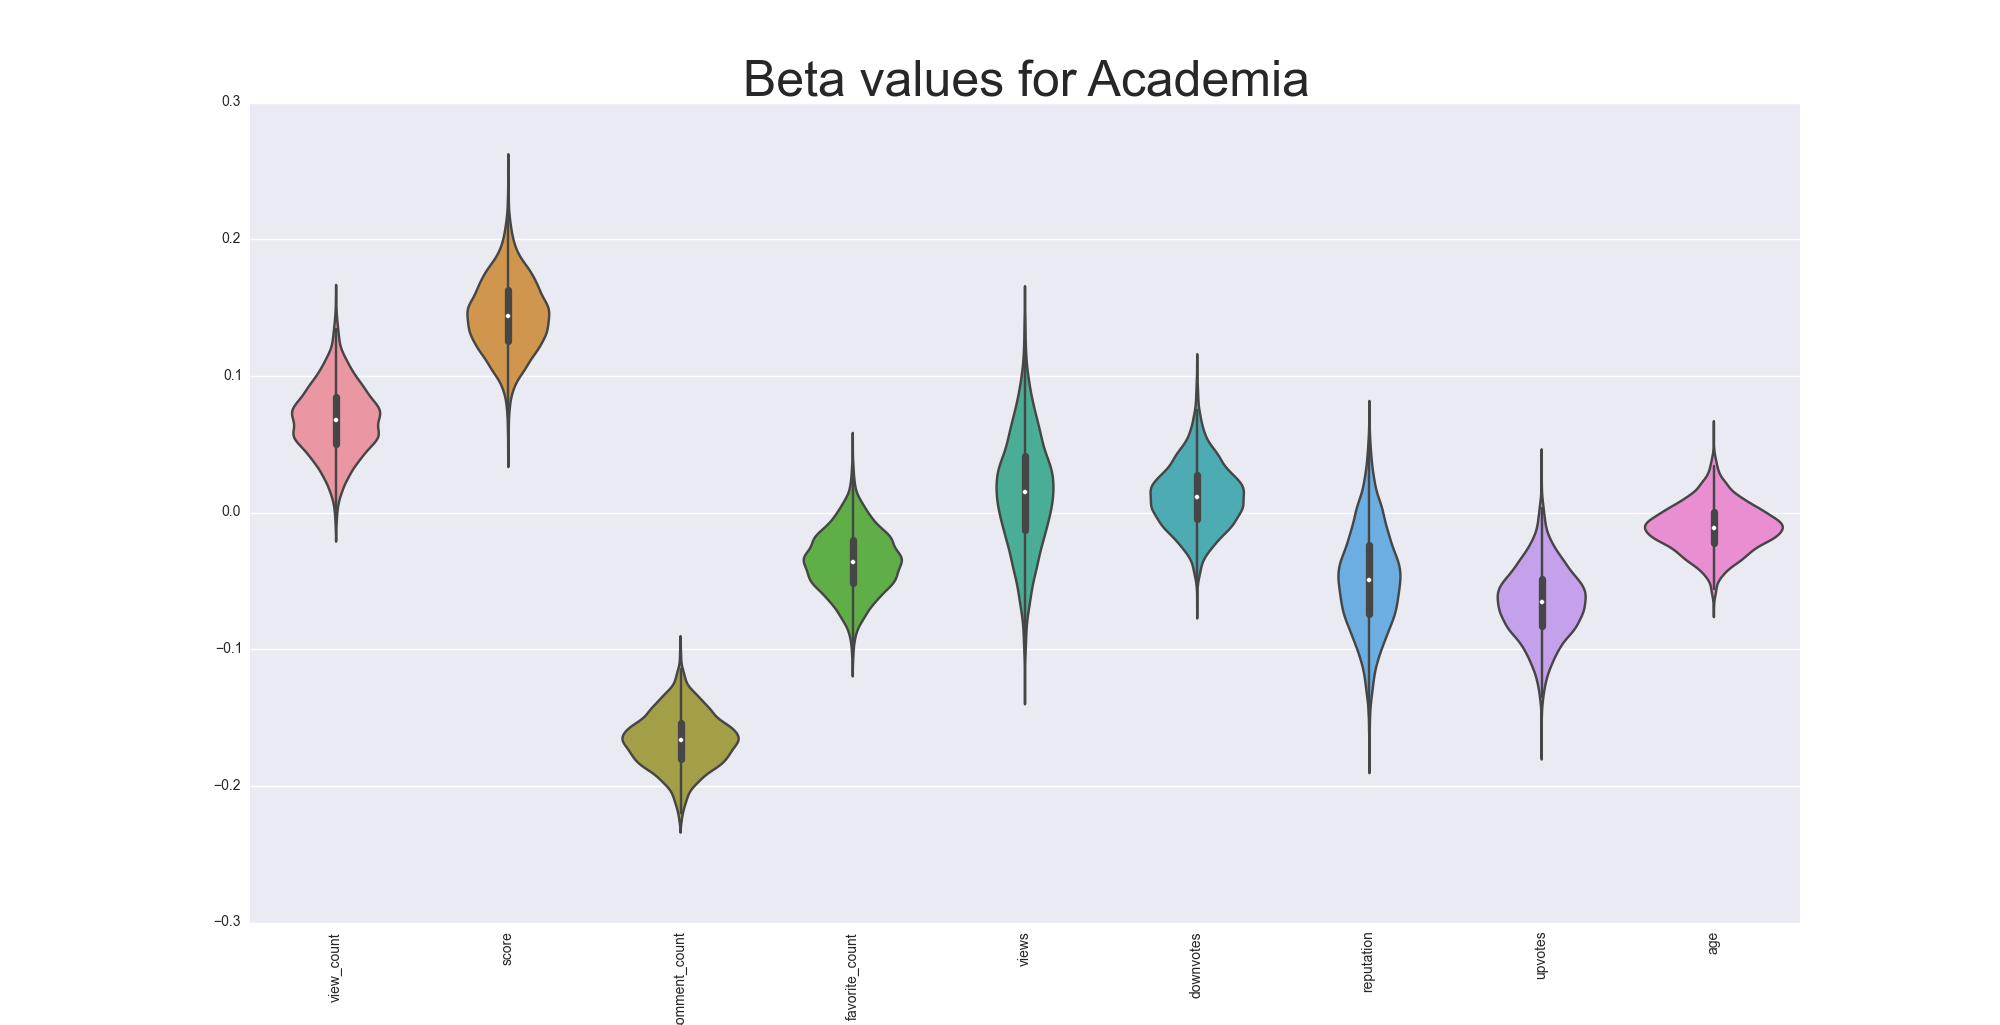
\includegraphics[scale = 0.25]{academia_violin.png}
  \caption{Academia Beta Values for Probit Regression}
  \label{vp_academia}
\end{figure}

\begin{figure}[h]
  \centering
  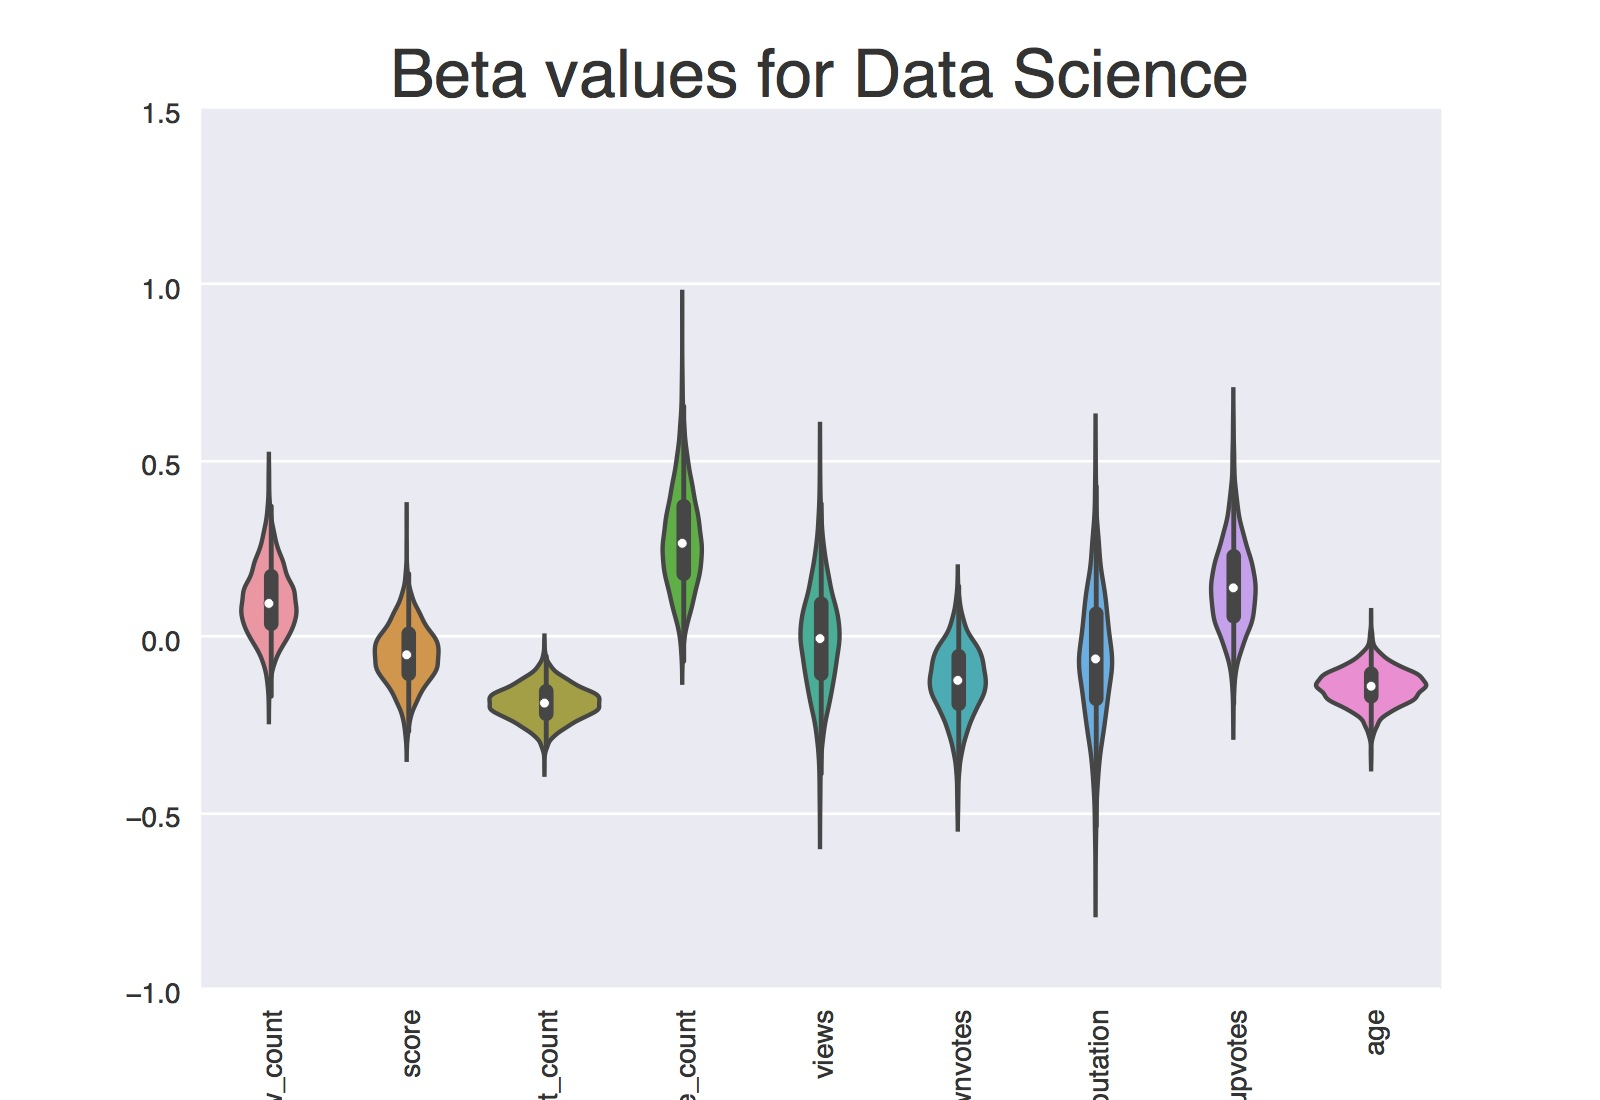
\includegraphics[scale = 0.3]{Data_science_vplot.jpg}
  \caption{Data Science Beta Values for Probit Regression}
  \label{vp_data_science}
\end{figure}

Because a higher regression coefficient in probit regression means that a variable raises the probability of a positive outcome, we can see that the observed values from Academia reinforce the patterns observed in the coefficients for standard and Bayesian linear regression. Specifically, view count and score have a strong positive impact on a question getting answered within four hours, and a high comment count has a negative impact. The impact of the rest of the parameters is relatively negligible. 

The coefficients for the Data Science stack exchange are less aligned with the results from the standard regression models. Comment count still has a strong negative impact on the regression, but the contribution of score and view count are less pronounced.

\section{Conclusion}

First, the results that we obtained were not particularly strong results. There are two possible conclusions to draw from this: the first is that we selected the wrong models, and the second is that the covariates we selected do not have strong predictive power for the amount of time it takes to answer a question. Exhaustive investigation of the other variables in the dataset would be a valid next step to determine whether the former or the latter is correct. 

Across all exchanges, having a high comment count on a post indicated that the question will take longer to get answered. We hypothesize the existence of two causes for this. First, that questions which are poorly framed will require clarification from commenters before they can be answered, and so those questions will have higher numbers of comments. Secondly, there may be some intrinsically difficult questions which simply require more comments to hash out an acceptable solution. It would be interesting to try some topic modeling on comments for questions with high comment count to see if they fall into one or both of these paradigms, or if something else is at work. Having a higher view count generally indicated a faster answer to a question. This also logically follows; if a question is seen by more participants, an answer is more likely to emerge. 

The strongest takeaway from this work is that in order to get a question answered on Stack Exchange, you simply have to ask a good question. By this, we mean that the features attached to a particular user did not have a strong impact on whether a question would or would not get answered. This is a good finding in that it shows Stack Exchanges are not particularly harsh towards outsiders asking questions; they are instead a viable source of information for anyone who's seeking it. 


% \pagebreak
\printbibliography


% --------------------------------------------------------------
%     You don't have to mess with anything below this line.
% --------------------------------------------------------------
\end{document}